\begin{titlepage} % larger: \huge, \Huge
\begin{center}
{\huge{\bf gstat user's manual}} \\
\vspace{.8cm}
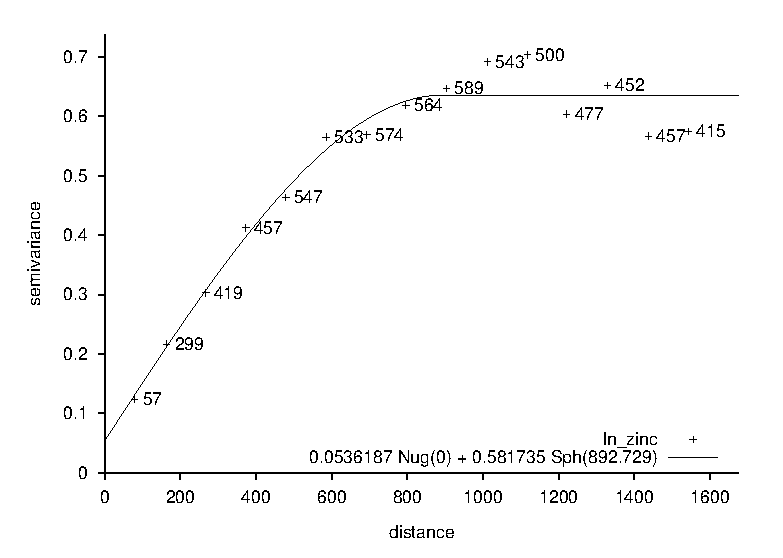
\includegraphics[scale=0.65]{\ext/vgm1} \\
\vspace{.4cm}
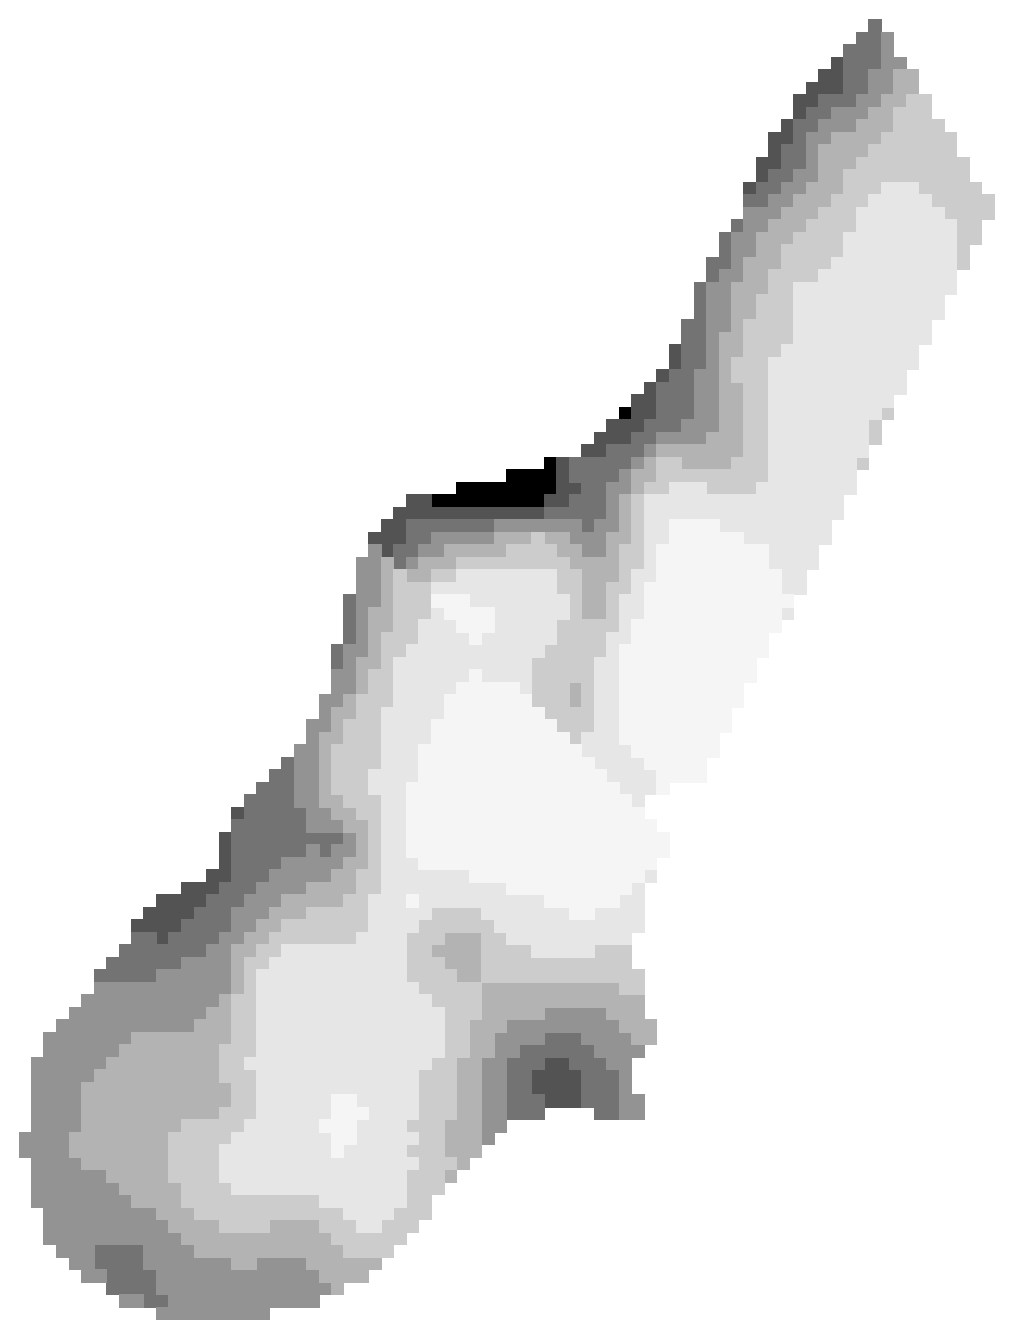
\includegraphics[scale=0.4]{\ext/lzn} \\
\vspace{.8cm}
{\em Edzer J. Pebesma} \\
Dept. of Physical Geography, Utrecht University \\
P.O. Box 80.115, 3508 TC, Utrecht, The Netherlands 
\end{center}

\newpage

\vspace*{\fill} % or try a length, 5c or \vspace*{\fill}

\noindent
gstat \version\ (\today) \\[2mm]
Copyright \copyright\ 1992, 2003 Edzer J. Pebesma \\ 
Permission is granted to copy, distribute and/or modify this document
under the terms of the GNU Free Documentation License, Version 1.2 or
any later version published by the Free Software Foundation; with no
Invariant Sections, no Front-Cover Texts, and no Back-Cover Texts. \\
See {\tt http://www.gnu.org/copyleft/fdl.html} \\[2mm]

Gstat is free software; you can redistribute it and/or modify it under
the terms of the GNU General Public License as published by the Free
Software Foundation; either version 2 of the License, or (at your
option) any later version. Gstat is distributed in the hope that it will
be useful, but without any warranty; without even the implied warranty
of merchantability or fitness for a particular purpose.  See the GNU
General Public License for more details. You should have received a copy
of the GNU General Public License along with the program (see the file
COPYING); if not, write to the Free Software Foundation, Inc., 675 Mass
Ave, Cambridge, MA 02139, USA. \\[2mm]
Meschach matrix library: Copyright \copyright\ 1993 David E. Stewart and
Zbigniew Leyk \\[2mm]
Gnuplot: Copyright \copyright\ 1986-1993, 1998 Thomas Williams and Colin 
Kelley and many others \\[2mm]
Relevant Internet locations:\\
Gstat: \http \\
Meschach: \code{ftp://ftpmaths.anu.edu.au/pub/meschach/meschach.html} \\
Gnuplot: \code{http://www.gnuplot.info/} \\
R: \code{http://www.r-project.org} \\
S-PLUS: \code{http://www.insightful.com}
\end{titlepage}
